\documentclass[12pt]{article}
\usepackage{lmodern}
\usepackage[T1]{fontenc}
\usepackage[dvips,letterpaper,margin=0.75in,bottom=0.75in]{geometry}
\usepackage{cancel}
\usepackage{graphicx}
\usepackage{braket}
\usepackage{latexsym,amssymb,amsmath}
\usepackage{pdfpages}
\usepackage{xcolor}
\usepackage{capt-of}
\usepackage{amsmath}
\usepackage{cite}
\newcommand{\tcr}{\textcolor{red}}
\newcommand{\tcb}{\textcolor{blue}}


\usepackage[american,fulldiode]{circuitikz}
\tikzset{component/.style={draw,thick,circle,fill=white,minimum size =0.75cm,inner sep=0pt}}

\begin{document}
\ctikzset{bipoles/thickness=1}
\ctikzset{bipoles/length=.6cm}


%%%%%%%%%%%%%%%%%%%%%%%%%%%%%%%%%%%%%%%%%%%%%%%%%%%%%%%%%%%%%%%%
%%%%%%%%%%%%%%%%%%%%%%%%%%%%%%%%%%%%%%%%%%%%%%%%%%%%%%%%%%%%%%%%
\title{Alternative Proposals for Anderson Road \\
  and Cesar Chavez Elementary School Improvements}
\author{Michael Mulhearn \\
(michaeljmulhearn@gmail.com)}
%%%%%%%%%%%%%%%%%%%%%%%%%%%%%%%%%%%%%%%%%%%%%%%%%%%%%%%%%%%%%%%%
%%%%%%%%%%%%%%%%%%%%%%%%%%%%%%%%%%%%%%%%%%%%%%%%%%%%%%%%%%%%%%%%

\maketitle

\section{Introduction}

The plans for Anderson Road and Cesar Chavez Elementary School (CCE)
improvement as presented to the community on Sept 11, 2025, are deeply
and fundamentally flawed.  The design does not align with the
priorities of the community.  As will be explained below, no single
segment of the community will be left unscathed by this design.  Going
forward, the author insists on more community involvement throughout
the process, particularly to develop design principles and priorities,
and explore top-level strategies.  Before any major infastrucure
changes are made, we need quantitative estimates followed by pilot
studies to validate those estimates and obtain community feedback.
This proposal will explain the flaws in the current design, suggest
design priorities and constraints, and suggests top-level strategies.
The proposal also presents some example design concepts which
demonstrate that the design priorities can be achieved within the
proposed design constraints.

\section{Flaws in the Presented Design}

No throughput calculations were presented at the meeting.  Without
employing valet's, the typical throughput of a single-lane curbside
passenger loading zone is 150-240 cars per hour.  In the twenty minute
peak drop-off period, that amounts to 30-80 cars.  That number might
seem unbelievably low upon first hearing it, and so it deservers some
explanation.  The best practice is to have a curbside pasenger loading
zone with a limited number of places and a longer single direction
queue to enter the loading zone.  Suppose there are four parking
spaces in the loading zone, in perfect continuous operation, with 30
seconds to park, and 30 seconds for the students to exit their
vehicle.  That would accommodate 240 cars per hour.  You might try to
have space for more than four vehicles in the loading zone, but extra
space at the front is not accessible to cars in the queue while cars
unload in the spots further back.  If you have ever sat in the back of
a large plane, you are familiar with this effect.  With professional
traffic management personel, one can do somewhat better than these
estimates, but why would we build out infrastructure that requires
increased personnel cost in perpetuity, unless we had no other choice?

By now it should be clear that during morning drop-off, the on-site
queue will fill immediately, and spill out into the surrounding area.
The proposed design dramatically exacerbates the problem by having
three competing entry paths into the queue: northbound on Anderson,
southbound on Anderson, and westbound on Rutgers.  These drivers are
going to be competing to maintain their place in the queue. This will
inevitably lead to counter-productive driver behavior, such as
blocking the intersection to hold one's place.  Here again, highly
active management (e.g. a police presence) can improve things, but why
would we implement a traffic design that creates these problems in the
first place?

So far, we have only considered community members who are dropping-off
students by motor vehicle, but the deep flaws in this design ripple
outward even further, negatively impacting everyone in the community.
An important consideration are the many UC Davis students that bike
past CCE on Anderson heading south.  In the current sytem, during
drop-off, southbound bike traffic follows a bike lane that is being
crossed by cars entering and exiting the loading zone.  No doubt this
was a driving consideration for this design, but it fails to improve
matters, due to the new four way intersection at Anderson and Rutgers.
To a bike driving along the upper edge of the ``T'', a three-way
intersection (the current configuration) is significantly safer than a
four-way intersection.  The proposed four-way intersection will be
occupied by frustrated drivers fighting for limited spots in a queue.
Drivers will push the limits of metering and traffic rules in order to
claim their spot in line, and bikers will be at grave risk.  What
about other bikers and walkers?  Driver frustruation is going to
inevitably lead some drivers to claim any available bike path as an
ad-hoc drop-off zone.  This will push bikes into traffic or onto
sidewalks, also negatively impacting walkers.

Implementing the presented design would negatively impact all of the
community members, and come at a high cost to other site
ammentities. Traffic is brought directly alongside the kindergarten
area, leaving parents nowhere to wait with their children.  One of the
few areas on site with natural shade, a seating area where we hold ice
cream socials and outdoor performances, would be converted into a
parking lot.  The CCE facade, currently presenting a modest, calm, and
symmetric parking lot, would be replaced by a sprawling and
irregularly shaped parking lot providing no effective buffer between
the drop-off chaos and school buildings.  {\bf This plan presented to
  the community on Septemeber 11, 2025 needs to be scrapped and
  reconsidered starting from a careful consideration of the
  community's priorities.}

\section{Proposed Design Priorities and Constraints}
\label{sec:priorities}

\begin{figure}[htbp]
  \centering
  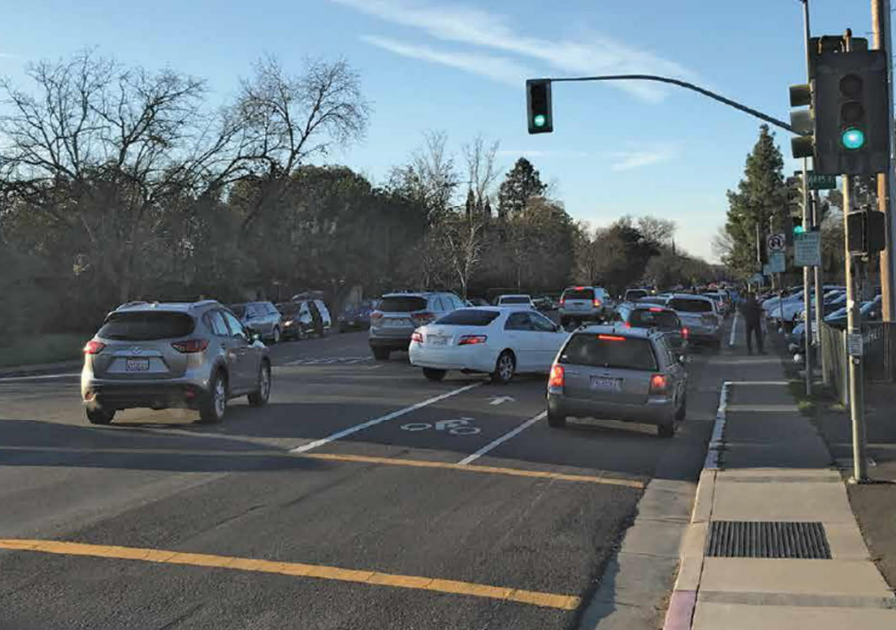
\includegraphics[width=0.7\textwidth]{existing.png}
  \caption{The existing curbside drop-off is quite chaotic, as shown
    in this photo presented in during the community workshop in 2020,
    but which could have been taken yesterday.}
  \label{fig:existing}
\end{figure}

The author proposes the following priorities all aimed at improving
safety for the community:
\begin{itemize}

\item The current system puts cyclist traveling southbound past CCE at
  risk, because cars must cross and recross the bike lane in order to
  pull into and out of the curbside loading zone.  The author
  considers improving this situation as the highest priority.  See
  Fig.~\ref{fig:existing}.
  
\item There are conflict points between walkers and cyclists, most
  notably in the vicinity of the intersection of Anderson and Rutgers.
  (See Fig.~\ref{fig:landing} below.)  The existing signaling and traffic
  guard do an excellent job of mitigating conflict between motor
  vehicles with pedestrians and cyclists, and we should not do
  anything to degrade that.

\item The current curbside passenger loading zone southbound on
  Anderson is chaotic.  If this chaos can be effectively reduced, we
  should do so, but only if it is not at grave cost to other more
  vulnerable members of the community.  We should also be realistic
  about how much the chaos can be reduced: drivers that choose to
  drive during peak times will inevitably encounter (and contribute
  to) traffic, and some inevitable chaos will ensue.

\end{itemize}
It is helpful to impose constraints on a design that support community
priorities and prevent inadvertent regressions while pursuing the
project priorities.  The author proposes the following constraints:

\begin{itemize}

\item {\bf No single tree will be cut down.}  Natural shade is a highly
  limited resource on the site, and there are plenty of alternatives
  to mitigate existing problems that do not require destroying any
  trees.

\item {\bf No additional on-site surfaces will be converted to
  motor-vehicle use.}  This principle avoids the classic design
  anti-pattern of over-accommodating motor vehicle drivers at the
  expense of other community members.

\item {\bf Do not accommodate on-site drop-off for northbound motor
  vehicles on Anderson.}  The site cannot accommodate these drivers at
  a reasonable cost to the rest of the community.  These drivers will
  need to plan their route to approach from the north or
  use off-site drop off.

\item {\bf Do not create any new four-way intersections.}  Pedestrian
  scramble can be an effective way to improve upon an existing
  four-way intersection, but it only mitigates problems. It is a much
  better approach to simply avoid having a four-way intersection in
  the first place.

\item {\bf Be quantitative.}  Estimate the throughput of various modes of
  traffic and compare it to the measured throughput of the existing
  system (the author has already begun collecting such data
  independently).  Conduct pilot studies to validate the quantitative
  estimates before investing in any signficant infastruture
  investments.
  
\end{itemize}

\section{Proposed Top-Level Strategies}

The author proposes a few different top-level strategies for
consideration:
\begin{itemize}

\item {\bf Minimalist Approach:} The existing system has some flaws,
  most noticible as the chaos during morning drop-off that most
  negatively impacts southbound cyclists on Anderson.  This approaches
  would attempt to mitigate these problems using only small
  incremental changes.

\item {\bf Realistic On-Site Drop-off Approach:} A carefully designed
  on-site drop-off could reduce chaos, but it must be realistic about
  throughput, and plan to accommodate the queue that will inevitably
  spill off site.  It should follow best practices for curbside
  passenger loading zones, most importantly, having one single access
  route (e.g. southbound on Anderson) to avoid conflicts.

\item {\bf Widen the Project Scope:} This approach would be more
  ambitious and consider Anderson, Oak, and Sycamore as part of an
  integrated traffic system that supports three schools sites and the
  surrounding communities in a choherent way.  This could include
  making roads one way, either during peak times or permanently, and
  other dynamic and transformative measures.  While the author
  encourages such big thinking for our city, it is beyond the scope of
  this proposal to flesh this out any further.
  
\end{itemize}


\section{Minimalist Design Concept}

\begin{figure}[htbp]
  \centering
  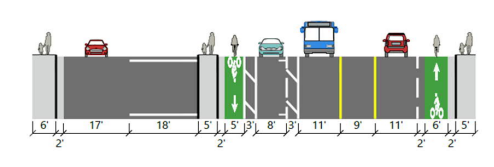
\includegraphics[width=0.5\textwidth]{concept1.png}
  \caption{In the Concept 1 presented to the community back in 2020, the bike lane
    is relocated to the right-hand side of the curbside drop-off
    vehicles.}
  \label{fig:concept1}
\end{figure}

\noindent
The existing infastructure has flaws but is serviceable, and we should
seriously consider a minimalist approach that makes only slight
changes necessary to achieve the priorities from
Section~\ref{sec:priorities}.  This approach would keep the existing
off-site curbside passenger loading zone unchanged, and would not
modify school property to accommodate on-site drop-off.  Central to
this approach is avoiding making any other upgrades to the site that
would trigger new requirements for major changes such as on-site
passenger loading zones.

The biggest problem in the present configuration is the crossing of
the bike lane with the curbside drop-off southbound on Anderson, as
illustrated in Fig.~\ref{fig:existing}.  The minimalist approach would
be to improve matters, particularly for cyclists, but leave the
loading zone in or near its present location.  The bike lane clearly
needs to be relocated.  In the Concept 1 presented to the community in
2020, the bike lane was simply relocated to the right-hand side of the
passenger loading zone, as shown in Fig.~\ref{fig:concept1}.  The
concept includes a three-foot buffer to mitigate conflict between
passengers being dropped off and the bikes.  Other relocations are
possible.  Using a pedestian scramble type signal, the southbound bike
lane could be moved across the street, alongside the northbound bike
lane, protected from on-coming traffic by parked cars or physical
barriers.  Another option is to redirect the bike lane into or around
the CCE parking lot.

\begin{figure}[htbp]
  \centering
  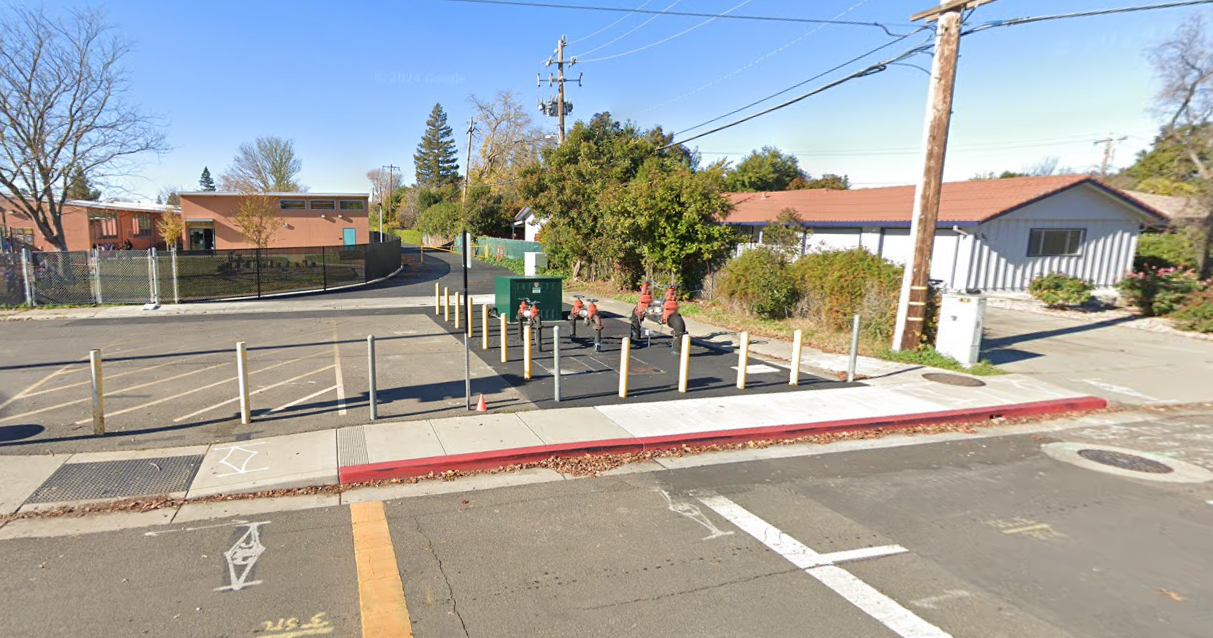
\includegraphics[width=0.8\textwidth]{landing.png}
  \caption{The westside landing at the intersection of Anderson and
    Rutgers.  Cyclist arriving at CCE are generally attempting to
    reach the black access road to the right of CCE, in order to reach
    the bike lock station, but they have no designated path.}
  \label{fig:landing}
\end{figure}

The second biggest safety issue arises from conflicts between cyclists
and pedestrians at the intersection of Rutgers and Anderson.  As shown
in Fig.~\ref{fig:landing}, cyclists arriving at CCE are generally
trying to reach the access road that leads to the bike lock station.
Generally, cyclists take two approaches, using the curb cuts to either
the left or right of the red curb shown in the picture.  If they go to
the left, they conflict with pedestians crossing Anderson or arriving
on campus from the north.  If they go to the right, they conflict with
pedestrians entering from the north at a particularly narrow and
awkward section of curbing.  Simple measures like widening the curb
cut and designating a bike lane, including a connection to the access
road alongside CCE, would dramatically improve the situation.  A
little paint goes a long way in this context.  Presumably, this is
also an emergency access corridor, but one can still imagine making
this space more aesthetically appealing by adding vegetation and shade
features, without disturbing any of the critical infastructure or
access.

The minimalist approach would leave the chaotic passenger loading zone
in its present off-site location. But with the bike lane relocated and
children exiting from curbside, the safety risk resulting from this
chaos is minimal.  The primary risk is low-speed collisions of motor
vehicles.  There are policy changes that CCE could make in order to
reduce peak demand and thus reduce the chaos.  Staggering student
arrival times by grade and having longer arrival time windows could
spread out the drop-off frenzy, calming some of the chaos.  Adding
additional off-site curbside passenger loading zones further away, but
still in easy walking distrance for older CCE students, would also
reduce congestion at the existing loading zone.

It should be understood that however chatoic the current loading zone
appears, it has higher throughput than all but the best managed
on-site single-lane passenger loading zones.  The chaos is from cars
leaving and exiting at multiple locations simultanously, allowing
throughput at a scale that an on-site drop-off at this site will never
be able to accommodate.  The chaos also encourages drivers to consider
other forms of transportation.


\section{Realistic On-Site Drop-off Design Concept}

\begin{figure}[htbp]
  \centering
  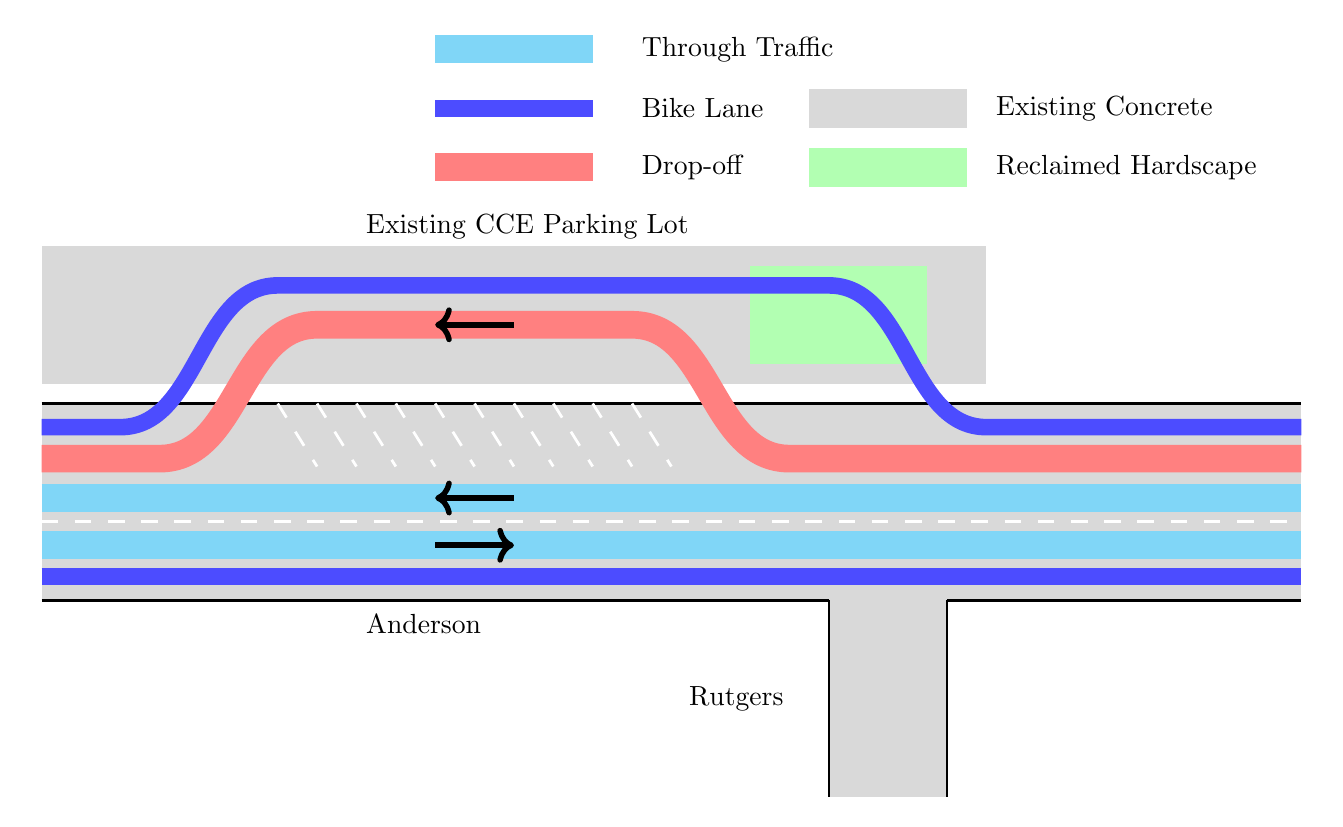
\begin{tikzpicture}[scale=1]
    % styles
    \tikzset{
      boundary/.style   = {line width=1pt, draw=black},
      roadfill/.style   = {fill=gray!30, draw=none},
      greenfill/.style   = {fill=green!30, draw=none},
      divider/.style    = {draw=white, line width=1pt, dash pattern=on 6pt off 6pt},
      bikelane/.style   = {line width=6pt, draw=blue!70},
      dropoff/.style    = {line width=10pt, draw=red!50},
      thrulane/.style   = {line width=10pt, draw=cyan!50},
      flowarrow/.style  = {->, line width=2pt, draw=black}
    }
    % Anderson and Rutgers Pavement:
    \path[roadfill] (-8,-1.5)  rectangle (8,1);
    \path[roadfill] (2, 0.5) rectangle (3.5,-4.0);
    \draw[boundary] (-8, 1)  -- (8,1);
    \draw[boundary] (-8, -1.5)  -- (2,-1.5);
    \draw[boundary] (3.5, -1.5) -- (8,-1.5);
    \draw[boundary] (2,-1.5) -- (2, -4);
    \draw[boundary] (3.5,-1.5) -- (3.5, -4);    

    % CCE parking lot:
    \path[roadfill] (-8, 1.25) rectangle (4,3);
    \path[greenfill] (1, 1.5) rectangle (3.25,2.75);
    
    \draw[bikelane]
    (-8,0.7) -- (-7,0.7)
    .. controls (-6,0.7) and (-6,2.5) .. (-5,2.5)
    -- (2,2.5)
    .. controls (3,2.5) and (3,0.7) .. (4,0.7)
    -- (8,0.7);

    \draw[bikelane]
    (-8,-1.2) -- (8,-1.2);
    

    \draw[dropoff]
    (-8,0.3) -- (-6.5,0.3)
    .. controls (-5.5, 0.3) and (-5.5,2.0) .. (-4.5,2.0)
    -- (-0.5,2.0)
    .. controls (0.5, 2.0) and (0.5,0.3) .. (1.5,0.3)
    -- (8, 0.3);


    % Through traffic:
    
    \draw[thrulane]
    (-8,-0.2) -- (8, -0.2);

    % Dividers:
    \draw[divider] (-8,-0.5) -- (8,-0.5);
    
    \draw[thrulane]
    (-8,-0.8) -- (8, -0.8);

    \draw[flowarrow] (-2, 2.0) -- (-3, 2.0);
    \draw[flowarrow] (-2,-0.2) -- (-3,-0.2);
    \draw[flowarrow] (-3,-0.8) -- (-2,-0.8);

    % Dividers:
    \draw[divider] (-5.0,1.0) -- (-4.5,0.2);
    \draw[divider] (-4.5,1.0) -- (-4.0,0.2);

    \draw[divider] (-4.0,1.0) -- (-3.5,0.2);
    \draw[divider] (-3.5,1.0) -- (-3.0,0.2);

    \draw[divider] (-3.0,1.0) -- (-2.5,0.2);
    \draw[divider] (-2.5,1.0) -- (-2.0,0.2);

    \draw[divider] (-2.0,1.0) -- (-1.5,0.2);
    \draw[divider] (-1.5,1.0) -- (-1.0,0.2);

    \draw[divider] (-1.0,1.0) -- (-0.5,0.2);
    \draw[divider] (-0.5,1.0) -- (-0.0,0.2);

    \path[roadfill] (1.75,4.5)  rectangle (3.75,5.0);
    \path[greenfill] (1.75,3.75)  rectangle (3.75,4.25);
    \node[anchor=west] at (4,4.75) {Existing Concrete};
    \node[anchor=west] at (4,4.00) {Reclaimed Hardscape};

    \draw[thrulane] (-3,5.50) -- (-1.0,5.50);
    \draw[bikelane] (-3,4.75) -- (-1.0,4.75);
    \draw[dropoff]  (-3,4.00) -- (-1.0,4.00);
    \node[anchor=west] at (-0.5, 5.50) {Through Traffic};
    \node[anchor=west] at (-0.5, 4.75) {Bike Lane};
    \node[anchor=west] at (-0.5, 4.00) {Drop-off};

    \node[anchor=west] at (-4,3.25) {Existing CCE Parking Lot};
    \node[anchor=west] at (-4,-1.8) {Anderson};
    \node[anchor=west] at (0.1,-2.75) {Rutgers};
    
  \end{tikzpicture}
  \caption{A proposal that accommodates an on-site drop-off. The essential
    feature is that entrance to the loading zone is limited to southbound
    traffic on Anderson, as the best way to accommodate the inevitable queue.}
  \label{fig:dropoff}
\end{figure}

\noindent
A design concept that implements an on-site passenger loading zone is
presented in Fig.~\ref{fig:dropoff}.  Anderson road at CCE currently
has three traffic lanes (including an under-utilized shared middle
lane) plus bike lanes, parking, and a curbside passenger loading zone.
This concept repurposes the shared middle lane as a dedicated through
lane for southbound traffic on Anderson.  This accommodates
through-lanes for both northbound and southbound traffic on Anderson
plus a dedicated lane for access to the CCE on-site drop-off.  The
entrance to the on-site drop-off is intentionally offset from the
intersection of Anderson and Rutgers in order to avoid creating a new
four-way intersection.  Access to the drop-off is also limited to
southbound vehicles on Anderson, in order to accommodate the
inevitable queue that will develop.  Physical barriers could be used
to prevent drivers from Rutgers or northbound drivers on Anderson from
attempting to enter.  To reduce demand on the on-site loading zone,
off-site passenger loading zones within easy walking distance for
older CCE students should be included in the design.

The bike lane is diverted in order to avoid crossing the path of the
drop-off traffic.  The space on Anderson freed up by relocating the
passenger loading zone and bike path can be repurposed as permitted
parallel or diagonal parking for CCE staff, in order to reclaim any
spaces lost in the existing parking space.  There is also under
utilized city property further south on Anderson which could
potentially accommodate additional parking for CCE and Redwood Park.

Nearly every community member benefits under this design concept.  The
largest beneficiaries are the southbound cycle traffic.  With a modest
diversion, they now circumvent the CCE drop-off chaos.  Northbound
through-traffic on Anderson, both motor vehicles and cycles, and
including right turns from Rutgers, are not significantly impacted.
Southbound through traffic now enjoys a dedicated through lane which
avoids the chaos during drop-off.  The dedicated left-turn lane for
Rutgers is lost\footnote{In fact, the dedicated left turn lane could
be maintained at the expense of some curbside parking spaces.}, but
this loss can be mitigated by prohibiting left turns onto Rutgers
during peak hours.  The neighborhood should benefit from calmer, less
chaotic drop-offs.  Pedestians are largely unaffected, as they are
already well protected from motor vehicle traffic by signaling and a
crossing guard.  The sidewalks on both sides of Anderson are not being
compromised.  However, they stand to benefit from better signaling and
an improved landing on the side opposite Rutgers.  In particular, the
dedicated bike lane should eliminate the present conflict between
pedestrians crossing Anderson and cyclists heading south or entering
CCE campus.  The design allows the north end of the CCE parking lot to
be reclaimed as a gathering space for humans, and should be improved
to include vegetation and shade, while perserving emergency access.

Most of the risk in this design stems from potential misbehavior by
drivers.  Attempts to access the drop-off from Rutgers or by a left
turn from northbound traffic on Anderson can be avoided by adding
physical barriers between the drop-off lane and the through lane all
the way through the intersection.  The on-site drop-off will
inevitably be slower than the current system, and this may lead more
drivers to use bike lanes, driveways, and bus stops as ad-hoc drop-off
locations.  This can be discouraged by moving bike lanes closer to the
curbs, behind parked cards, and by bumping out bus stops.  Some
drivers may attempt to use free spots amongst the new parking on
Anderson for drop off. This can be discouraged by making sure these
spots are designated and enforced as permit only and no stopping.  The
constriction of through traffic at CCE should naturally slow traffic,
but additional traffic calming measures could be added for this
highly congested area.

Given the space limitations, on-site passenger loading at CCE will be of
limited capacity, and a queue will inevitably spill out into the
neighborhood.  Quantitative estimates for any design, a plan for
accommodating the queue, and managing neighborhood expectations
regarding the queue will be essential.  It is entirely possible that
removing the existing chaotic (and yet effective) curbside parking
will make conditions dramatically worse in the neighborhood, and so a
pilot study is absolutely essential.

\section{Conclusion}

This proposal is obviously no replacement for the work of professional
civil and traffic engineers.  Instead, it is aimed at refocussing
those efforts in directions that are more responsive to our
community's needs.  The presented design concepts illustrate that it
should be possible to address the communities priorities while
remaining within the community-preservering design constraints.  We
don't want to tear down any of our few remaining shade trees.  We don't want
our drop-off traffic queue to spread frustration and chaos into our
neighborhood.  And we do not need too.  We can have safe streets,
calmer drop-offs, shady trees, and appealing public spaces.  In fact,
we insist on it!

\end{document}

